\documentclass[aspectratio=169,10pt]{beamer}

% Shared Beamer setup for Fall 2026 course slides.
% Clean Cal Poly-inspired theme: no custom class files or uncommon packages.
\mode<presentation>{
  \usetheme{default}
  \usefonttheme{professionalfonts}
}

\definecolor{CalPolyGreen}{HTML}{154734}
\definecolor{CalPolyGold}{HTML}{BD8B13}
\definecolor{CalPolySage}{HTML}{7FA28F}
\definecolor{CalPolyMint}{HTML}{DDF1E7}
\definecolor{CalPolySand}{HTML}{A29F86}
\definecolor{CalPolyBeige}{HTML}{EFEEDE}
\definecolor{DeckInk}{HTML}{1F2933}
\definecolor{DeckMuted}{HTML}{5F6B7A}
\definecolor{DeckSoft}{HTML}{F7F7F5}

\setbeamersize{text margin left=0.55in,text margin right=0.55in}
\setbeamercolor{normal text}{fg=DeckInk,bg=white}
\setbeamercolor{structure}{fg=CalPolyGreen}
\setbeamercolor{title}{fg=white}
\setbeamercolor{frametitle}{fg=CalPolyGreen,bg=white}
\setbeamercolor{block title}{bg=CalPolySage,fg=white}
\setbeamercolor{block body}{bg=CalPolyMint,fg=black}
\setbeamercolor{alerted text}{fg=CalPolyGold}

\setbeamerfont{title}{size=\Huge,series=\bfseries}
\setbeamerfont{frametitle}{size=\Large,series=\bfseries}
\setbeamerfont{block title}{size=\normalsize,series=\bfseries}

\setbeamertemplate{navigation symbols}{}
\setbeamertemplate{itemize item}{\color{CalPolyGold}$\blacktriangleright$}
\setbeamertemplate{itemize subitem}{\color{CalPolyGreen}$\bullet$}
\setbeamertemplate{footline}{
  \hfill{\color{DeckMuted}\scriptsize\insertframenumber/\inserttotalframenumber}
  \hspace{0.18in}\vspace{0.12in}
}
\setbeamertemplate{frametitle}{
  \vspace{0.18in}
  \hspace{0.02in}\insertframetitle\par
  \vspace{0.08in}
  \noindent\makebox[\linewidth][l]{%
    {\color{CalPolyGold}\rule{0.55in}{2pt}}%
    {\color{CalPolyGreen}\rule{\dimexpr\linewidth-0.55in\relax}{2pt}}%
  }
}

\newcommand{\CourseNumber}{Course}
\newcommand{\CourseTitle}{Course Title}
\newcommand{\LectureNumber}{0}
\newcommand{\LectureTitle}{Lecture Title}
\newcommand{\LectureDate}{Date}
\newcommand{\CourseUnit}{Unit}

\newcommand{\coursenumber}[1]{\renewcommand{\CourseNumber}{#1}}
\newcommand{\coursetitle}[1]{\renewcommand{\CourseTitle}{#1}}
\newcommand{\lecturenumber}[1]{\renewcommand{\LectureNumber}{#1}}
\newcommand{\lecturetitle}[1]{\renewcommand{\LectureTitle}{#1}}
\newcommand{\lecturedate}[1]{\renewcommand{\LectureDate}{#1}}
\newcommand{\courseunit}[1]{\renewcommand{\CourseUnit}{#1}}

\author{Kirk Duran}
\institute{California Polytechnic State University, San Luis Obispo}
\date{\LectureDate}

\newcommand{\makedecktitle}{
  \begingroup
  \setbeamercolor{background canvas}{bg=CalPolyGreen}
  \begin{frame}[plain]
    \vfill
    \begin{center}
      {\usebeamerfont{title}\color{white}\LectureTitle\par}
      \vspace{0.18in}
      {\Large\color{white}Lecture \LectureNumber\par}
    \end{center}
    \vfill
    \noindent{\color{white}\rule{\linewidth}{1.2pt}}\par
    \vspace{0.08in}
    \noindent\colorbox{CalPolyGold}{\makebox[0.24\linewidth][c]{\color{white}\Large\CourseNumber}}
    \hspace{0.12in}{\color{white}\Large Kirk Duran}
  \end{frame}
  \endgroup
}

\newenvironment{keyidea}{\begin{block}{Key idea}}{\end{block}}
\newenvironment{activity}{\begin{block}{In class}}{\end{block}}
\newenvironment{cpdefinition}{\begin{block}{Definition}}{\end{block}}
\newenvironment{exampleblockcp}{
  \begingroup
  \setbeamercolor{block title}{bg=CalPolySand,fg=white}
  \setbeamercolor{block body}{bg=CalPolyBeige,fg=black}
  \begin{block}{Example}
}{
  \end{block}
  \endgroup
}

\newcommand{\imageplaceholder}[2][0.3in]{%
  \noindent\makebox[\linewidth][c]{%
    \fcolorbox{CalPolySage}{CalPolyBeige}{%
      \parbox[c][#1][c]{0.86\linewidth}{%
        \centering
        {\color{DeckMuted}\scriptsize Image placeholder: }%
        {\color{DeckInk}\scriptsize\ttfamily\detokenize{#2}}%
      }%
    }%
  }%
}

\newcommand{\sectionframe}[1]{
  \begingroup
  \setbeamercolor{background canvas}{bg=CalPolyGreen}
  \begin{frame}[plain]
    \vfill
    {\color{white}\LARGE\bfseries #1\par}
    \vspace{0.18in}
    {\color{CalPolyGold}\rule{0.22\paperwidth}{3pt}}
    {\color{white}\rule{0.62\paperwidth}{3pt}}
    \vfill
  \end{frame}
  \endgroup
}

\newcommand{\placeholdernote}{
  \begin{block}{Placeholder}
    Replace these bullets with the final lecture material, examples, and in-class activities.
  \end{block}
}


\usepackage{tikz}

\graphicspath{{../assets/lecture-17/}}

% If an image file is not yet available, skip the visual slot.
\newcommand{\lectureimage}[2][1.75in]{%
  \IfFileExists{../assets/lecture-17/#2}{%
    \includegraphics[width=\linewidth,height=#1,keepaspectratio]{#2}%
  }{}%
}

% Explicit placeholder for visuals/examples that will be added later.
\newcommand{\lectureplaceholder}[2][2.35in]{%
  \begin{center}
    \fbox{%
      \begin{minipage}[c][#1][c]{0.90\linewidth}
        \centering
        \small\textit{#2}
      \end{minipage}%
    }
  \end{center}%
}

\setbeamersize{text margin left=0.42in,text margin right=0.42in}

\coursenumber{CS 4880}
\coursetitle{Artificial Intelligence}
\lecturenumber{16}
\lecturetitle{First-Order Logic Inference}
\lecturedate{October 5, 2026}
\courseunit{Logic and Knowledge Representation}

\begin{document}

% Estimated pacing: 50 minutes
% Motivation and substitution: 9 min
% Unification and MGU: 17 min
% Generalized Modus Ponens: 8 min
% Forward/backward chaining: 12 min
% Limits and synthesis: 4 min

% -----------------------------------------------------------------------------
% Slide 1
% -----------------------------------------------------------------------------
\makedecktitle

\section{From Representation to Inference}

% -----------------------------------------------------------------------------
% Slide 2
% -----------------------------------------------------------------------------
\begin{frame}[shrink=10]{Representation Is Only Half the Job}
  \begin{columns}[T,onlytextwidth]
    \begin{column}{0.54\textwidth}
      Last time we gave the agent a richer language:
      \begin{itemize}
        \item objects and variables;
        \item predicates and relations;
        \item functions and nested terms;
        \item universal and existential rules.
      \end{itemize}

      But a knowledge base is useful only if the agent can \emph{derive new facts} from those general rules.
    \end{column}
    \begin{column}{0.40\textwidth}
      \lectureimage[2.70in]{slide2.png}
    \end{column}
  \end{columns}
  \begin{keyidea}
    First-order inference asks how general symbolic rules become concrete conclusions about particular objects.
  \end{keyidea}
\end{frame}

% -----------------------------------------------------------------------------
% Slide 3
% -----------------------------------------------------------------------------
\begin{frame}[shrink=10]{The Human Step We Need to Automate}
  Suppose the knowledge base contains
  \[
    \forall x\; Human(x) \rightarrow Mortal(x)
  \]
  and
  \[
    Human(Socrates).
  \]

  We immediately conclude
  \[
    Mortal(Socrates).
  \]

  \begin{block}{What did your brain silently do?}
    It noticed that the variable $x$ in the rule can stand for $Socrates$.
  \end{block}

  \begin{keyidea}
    The core computational problem is matching variable-containing expressions to specific terms.
  \end{keyidea}
\end{frame}

% -----------------------------------------------------------------------------
% Slide 4
% -----------------------------------------------------------------------------
\begin{frame}[shrink=10]{Three Pieces of First-Order Inference}
  \begin{columns}[T,onlytextwidth]
    \begin{column}{0.30\textwidth}
      \begin{block}{1. Substitution}
        Replace variables with terms in a consistent way.
      \end{block}
    \end{column}
    \begin{column}{0.30\textwidth}
      \begin{block}{2. Unification}
        Find substitutions that make expressions match.
      \end{block}
    \end{column}
    \begin{column}{0.30\textwidth}
      \begin{block}{3. Inference}
        Apply matched rules to derive new knowledge.
      \end{block}
    \end{column}
  \end{columns}

  \lectureimage[1.70in]{slide4.png}

  \begin{keyidea}
    Unification is the bridge between representation and automated reasoning.
  \end{keyidea}
\end{frame}

\section{Substitution}

% -----------------------------------------------------------------------------
% Slide 5
% -----------------------------------------------------------------------------
\begin{frame}[shrink=10]{Substitution: Giving Variables Concrete Values}
  A \textbf{substitution} is a mapping from variables to terms.

  \[
    \theta = \{x/Socrates\}
  \]

  means ``replace $x$ with $Socrates$.''

  Applying $\theta$ to a sentence:
  \[
    Human(x)\theta = Human(Socrates).
  \]

  \begin{keyidea}
    A substitution does not change the rule's meaning; it creates one particular instance of a general pattern.
  \end{keyidea}
\end{frame}

% -----------------------------------------------------------------------------
% Slide 6
% -----------------------------------------------------------------------------
\begin{frame}[shrink=10]{Substitutions Can Bind Several Variables}
  Consider
  \[
    \theta = \{x/Alice,\;y/Room214\}.
  \]

  Then
  \[
    In(x,y)\theta = In(Alice,Room214).
  \]

  and
  \[
    Connected(y,Hallway2)\theta = Connected(Room214,Hallway2).
  \]

  \begin{keyidea}
    The same substitution must be applied consistently everywhere the bound variable appears.
  \end{keyidea}
\end{frame}

% -----------------------------------------------------------------------------
% Slide 7
% -----------------------------------------------------------------------------
\begin{frame}[shrink=10]{Substitution Works Inside Nested Terms}
  Suppose
  \[
    \theta = \{x/Alice\}.
  \]

  Then
  \[
    SupervisorOf(x)\theta = SupervisorOf(Alice)
  \]

  and
  \[
    Knows(x,SupervisorOf(x))\theta
    = Knows(Alice,SupervisorOf(Alice)).
  \]

  \begin{keyidea}
    Substitution recursively replaces variables wherever they occur inside a term or sentence.
  \end{keyidea}
\end{frame}

% -----------------------------------------------------------------------------
% Slide 8
% -----------------------------------------------------------------------------
\begin{frame}[shrink=10]{Ground Expressions Have No Variables}
  \begin{columns}[T,onlytextwidth]
    \begin{column}{0.47\textwidth}
      \begin{block}{Contains variables}
        \[
          Carries(r,p)
        \]
        \[
          In(r,LocationOf(p))
        \]
      \end{block}
    \end{column}
    \begin{column}{0.47\textwidth}
      \begin{block}{Ground}
        \[
          Carries(Robot7,PackageA)
        \]
        \[
          In(Robot7,Room214)
        \]
      \end{block}
    \end{column}
  \end{columns}

  \begin{keyidea}
    A ground sentence refers only to specific terms; no variable bindings remain to be chosen.
  \end{keyidea}
\end{frame}

% -----------------------------------------------------------------------------
% Slide 9
% -----------------------------------------------------------------------------
\begin{frame}[shrink=10]{Pattern Matching Is the Simplest Case}
  A rule may contain a pattern such as
  \[
    Carries(r,p).
  \]

  A fact may be
  \[
    Carries(Robot7,PackageA).
  \]

  Matching discovers
  \[
    \theta = \{r/Robot7,\;p/PackageA\}.
  \]

  \begin{keyidea}
    Pattern matching asks which variable bindings make a template identical to a concrete expression.
  \end{keyidea}
\end{frame}

% -----------------------------------------------------------------------------
% Slide 10
% -----------------------------------------------------------------------------
\begin{frame}[shrink=10]{A Match Can Fail Immediately}
  Try to match
  \[
    In(Robot7,x)
  \]
  with
  \[
    In(Robot9,Room214).
  \]

  The first arguments are different constants:
  \[
    Robot7 \neq Robot9.
  \]

  No substitution for $x$ can repair that mismatch.

  \begin{keyidea}
    Variables can be bound; distinct constants cannot simply be rewritten to match each other.
  \end{keyidea}
\end{frame}

\section{Unification}

% -----------------------------------------------------------------------------
% Slide 11
% -----------------------------------------------------------------------------
\begin{frame}[shrink=10]{Unification Generalizes Pattern Matching}
  \begin{cpdefinition}
    \textbf{Unification} finds a substitution that makes two first-order expressions syntactically identical.
  \end{cpdefinition}

  Example:
  \[
    Knows(Alice,x)
  \]
  and
  \[
    Knows(y,Bob)
  \]

  unify under
  \[
    \theta = \{y/Alice,\;x/Bob\}.
  \]

  \begin{keyidea}
    Both sides may contain variables; unification solves the bindings jointly.
  \end{keyidea}
\end{frame}

% -----------------------------------------------------------------------------
% Slide 12
% -----------------------------------------------------------------------------
\begin{frame}[shrink=10]{Unification Must Respect Structure}
  To unify
  \[
    Parent(x,y)
  \]
  with
  \[
    Parent(Alice,Bob),
  \]
  we compare corresponding pieces:
  \[
    x \leftrightarrow Alice,
    \qquad
    y \leftrightarrow Bob.
  \]

  So
  \[
    \theta = \{x/Alice,\;y/Bob\}.
  \]

  \begin{keyidea}
    Predicate names, function names, arity, and argument positions must all line up.
  \end{keyidea}
\end{frame}

% -----------------------------------------------------------------------------
% Slide 13
% -----------------------------------------------------------------------------
\begin{frame}[shrink=10]{Repeated Variables Create Constraints}
  Can these expressions unify?
  \[
    Likes(x,x)
  \]
  \[
    Likes(Alice,Bob)
  \]

  The first argument requires
  \[
    x=Alice,
  \]
  while the second requires
  \[
    x=Bob.
  \]

  If $Alice\neq Bob$, no consistent substitution exists.

  \begin{keyidea}
    One variable must have one consistent binding throughout the expression.
  \end{keyidea}
\end{frame}

% -----------------------------------------------------------------------------
% Slide 14
% -----------------------------------------------------------------------------
\begin{frame}[shrink=10]{Functions Unify by Their Internal Structure}
  Consider
  \[
    Knows(x,MotherOf(x))
  \]
  and
  \[
    Knows(Alice,MotherOf(Alice)).
  \]

  The first arguments suggest
  \[
    x=Alice.
  \]

  The second arguments then become identical automatically.

  \[
    \theta = \{x/Alice\}.
  \]

  \begin{keyidea}
    Compound terms unify recursively: first the outer function, then its arguments.
  \end{keyidea}
\end{frame}

% -----------------------------------------------------------------------------
% Slide 15
% -----------------------------------------------------------------------------
\begin{frame}[shrink=10]{Nested Terms Can Force More Bindings}
  Unify
  \[
    Knows(x,SupervisorOf(y))
  \]
  with
  \[
    Knows(Alice,SupervisorOf(Bob)).
  \]

  Matching the structure yields
  \[
    x=Alice,
    \qquad
    y=Bob.
  \]

  Therefore
  \[
    \theta=\{x/Alice,\;y/Bob\}.
  \]

  \begin{keyidea}
    Unification decomposes complex expressions until it reaches variable-term bindings or a contradiction.
  \end{keyidea}
\end{frame}

% -----------------------------------------------------------------------------
% Slide 16
% -----------------------------------------------------------------------------
\begin{frame}[shrink=10]{Some Structures Can Never Unify}
  \begin{columns}[T,onlytextwidth]
    \begin{column}{0.47\textwidth}
      \begin{block}{Different predicate}
        \[
          Likes(Alice,x)
        \]
        \[
          Knows(Alice,Bob)
        \]

        Fail: $Likes \neq Knows$.
      \end{block}
    \end{column}
    \begin{column}{0.47\textwidth}
      \begin{block}{Different function}
        \[
          OwnerOf(x)
        \]
        \[
          SupervisorOf(Alice)
        \]

        Fail: function symbols differ.
      \end{block}
    \end{column}
  \end{columns}

  \begin{keyidea}
    Unification changes variable bindings, not the fixed symbolic structure of the language.
  \end{keyidea}
\end{frame}

% -----------------------------------------------------------------------------
% Slide 17
% -----------------------------------------------------------------------------
\begin{frame}[shrink=10]{The Occurs Check Prevents Circular Terms}
  Suppose we try to unify
  \[
    x
  \]
  with
  \[
    ParentOf(x).
  \]

  Naively binding $x/ParentOf(x)$ would make $x$ contain itself forever:
  \[
    x = ParentOf(ParentOf(ParentOf(\cdots))).
  \]

  A standard unification algorithm rejects this with the \textbf{occurs check}.

  \begin{keyidea}
    A variable cannot be bound to a term that already contains that same variable.
  \end{keyidea}
\end{frame}

% -----------------------------------------------------------------------------
% Slide 18
% -----------------------------------------------------------------------------
\begin{frame}[shrink=10]{The Most General Unifier}
  Often many substitutions can make expressions match.

  For
  \[
    Likes(x,IceCream)
  \]
  and
  \[
    Likes(Alice,y),
  \]
  the useful substitution is
  \[
    \theta = \{x/Alice,\;y/IceCream\}.
  \]

  A \textbf{most general unifier (MGU)} makes only the bindings necessary to force the match.

  \begin{keyidea}
    The MGU preserves as much freedom as possible instead of inventing unnecessary commitments.
  \end{keyidea}
\end{frame}

% -----------------------------------------------------------------------------
% Slide 19
% -----------------------------------------------------------------------------
\begin{frame}[shrink=10]{Why ``Most General'' Matters}
  Suppose
  \[
    Knows(x,y)
  \]
  must unify with
  \[
    Knows(Alice,z).
  \]

  One MGU is
  \[
    \theta = \{x/Alice,\;y/z\}.
  \]

  We do \emph{not} need to decide what $z$ is yet.

  \begin{keyidea}
    Keeping unresolved variables unresolved lets the result participate in later inference without losing valid possibilities.
  \end{keyidea}
\end{frame}

% -----------------------------------------------------------------------------
% Slide 20
% -----------------------------------------------------------------------------
\begin{frame}[shrink=12]{Unification as an Algorithm}
  \begin{block}{High-level idea}
  \ttfamily\small
  UNIFY(x, y, $\theta$)\\
  \quad if $\theta$ is failure: return failure\\
  \quad if x = y: return $\theta$\\
  \quad if x is a variable: UNIFY\_VAR(x, y, $\theta$)\\
  \quad if y is a variable: UNIFY\_VAR(y, x, $\theta$)\\
  \quad if both are compound with same operator:\\
  \qquad unify corresponding arguments recursively\\
  \quad else: return failure
  \end{block}

  \begin{keyidea}
    Unification is a recursive structural comparison that accumulates variable bindings as it descends.
  \end{keyidea}
\end{frame}

% -----------------------------------------------------------------------------
% Slide 21
% -----------------------------------------------------------------------------
\begin{frame}[shrink=10]{Worked Unification: Start with the Outer Structure}
  Unify
  \[
    Knows(x,SupervisorOf(y))
  \]
  with
  \[
    Knows(Alice,SupervisorOf(Bob)).
  \]

  Both use the predicate $Knows$ with two arguments, so compare arguments pairwise:
  \[
    x \;\text{with}\; Alice
  \]
  and
  \[
    SupervisorOf(y) \;\text{with}\; SupervisorOf(Bob).
  \]

  \begin{keyidea}
    Matching the outer symbol lets the algorithm safely recurse into corresponding arguments.
  \end{keyidea}
\end{frame}

% -----------------------------------------------------------------------------
% Slide 22
% -----------------------------------------------------------------------------
\begin{frame}[shrink=10]{Worked Unification: Accumulate Bindings}
  First pair:
  \[
    x \;\text{with}\; Alice
  \]
  gives
  \[
    \theta_1 = \{x/Alice\}.
  \]

  Second pair has matching function symbol $SupervisorOf$, so compare
  \[
    y \;\text{with}\; Bob.
  \]

  This extends the substitution:
  \[
    \theta_2 = \{x/Alice,\;y/Bob\}.
  \]

  \begin{keyidea}
    The substitution grows as constraints are discovered.
  \end{keyidea}
\end{frame}

% -----------------------------------------------------------------------------
% Slide 23
% -----------------------------------------------------------------------------
\begin{frame}[shrink=10]{Worked Unification: Verify the Result}
  Apply
  \[
    \theta = \{x/Alice,\;y/Bob\}
  \]
  to the first expression:
  \[
    Knows(x,SupervisorOf(y))\theta
  \]
  \[
    = Knows(Alice,SupervisorOf(Bob)).
  \]

  It is now identical to the second expression.

  \begin{keyidea}
    A candidate unifier is correct exactly when applying it makes the two expressions the same.
  \end{keyidea}
\end{frame}

\section{Generalized Modus Ponens}

% -----------------------------------------------------------------------------
% Slide 24
% -----------------------------------------------------------------------------
\begin{frame}[shrink=10]{From Matching to Inference}
  Propositional modus ponens says
  \[
    P,
    \qquad
    P\rightarrow Q
    \quad\Longrightarrow\quad
    Q.
  \]

  First-order rules contain variables, so we need to match the premises to known facts before firing the rule.

  \begin{keyidea}
    Generalized Modus Ponens adds unification to the familiar rule ``premises imply conclusion.''
  \end{keyidea}
\end{frame}

% -----------------------------------------------------------------------------
% Slide 25
% -----------------------------------------------------------------------------
\begin{frame}[shrink=10]{Generalized Modus Ponens}
  Suppose the rule is
  \[
    P_1 \land P_2 \land \cdots \land P_n \rightarrow Q.
  \]

  If a substitution $\theta$ makes every premise match known facts, infer
  \[
    Q\theta.
  \]

  \begin{cpdefinition}
    Generalized Modus Ponens applies a first-order rule after unifying its premises with facts in the knowledge base.
  \end{cpdefinition}

  \begin{keyidea}
    Unification chooses the instance; the inference rule produces the conclusion.
  \end{keyidea}
\end{frame}

% -----------------------------------------------------------------------------
% Slide 26
% -----------------------------------------------------------------------------
\begin{frame}[shrink=10]{Classic Example: King + Greedy $\Rightarrow$ Evil}
  Rule:
  \[
    King(x) \land Greedy(x) \rightarrow Evil(x).
  \]

  Facts:
  \[
    King(John),
    \qquad
    Greedy(John).
  \]

  Unifier:
  \[
    \theta = \{x/John\}.
  \]

  Therefore:
  \[
    Evil(John).
  \]

  \begin{keyidea}
    One general rule can fire for any object whose facts satisfy its premises.
  \end{keyidea}
\end{frame}

% -----------------------------------------------------------------------------
% Slide 27
% -----------------------------------------------------------------------------
\begin{frame}[shrink=10]{Campus Robot Rule}
  Suppose the robot uses
  \[
    Robot(r) \land Carries(r,p) \land Fragile(p)
    \rightarrow MoveSlowly(r).
  \]

  The KB contains
  \[
    Robot(Robot7),
  \]
  \[
    Carries(Robot7,PackageA),
  \]
  \[
    Fragile(PackageA).
  \]

  Matching all three premises gives
  \[
    \theta=\{r/Robot7,\;p/PackageA\}.
  \]

  \begin{keyidea}
    Multi-premise rules require one substitution that satisfies the premises consistently together.
  \end{keyidea}
\end{frame}

% -----------------------------------------------------------------------------
% Slide 28
% -----------------------------------------------------------------------------
\begin{frame}[shrink=10]{The Rule Fires with the Same Substitution}
  Apply
  \[
    \theta=\{r/Robot7,\;p/PackageA\}
  \]
  to the conclusion:
  \[
    MoveSlowly(r)\theta
    = MoveSlowly(Robot7).
  \]

  The new fact can now be added to the knowledge base.

  \begin{keyidea}
    The variable bindings discovered while matching the premises are reused to instantiate the conclusion.
  \end{keyidea}
\end{frame}

\section{First-Order Forward Chaining}

% -----------------------------------------------------------------------------
% Slide 29
% -----------------------------------------------------------------------------
\begin{frame}[shrink=10]{Forward Chaining Still Works---Now with Unification}
  \begin{enumerate}
    \item Start with known facts.
    \item Find a rule whose premises can unify with facts in the KB.
    \item Apply the resulting substitution to the conclusion.
    \item Add the new fact if it is not already known.
    \item Repeat until the query is found or no new facts appear.
  \end{enumerate}

  \begin{keyidea}
    Propositional forward chaining becomes first-order forward chaining by replacing exact premise matching with unification.
  \end{keyidea}
\end{frame}

% -----------------------------------------------------------------------------
% Slide 30
% -----------------------------------------------------------------------------
\begin{frame}[shrink=10]{Forward Chaining Example: Initial Knowledge}
  Facts:
  \[
    Robot(Robot7)
  \]
  \[
    Carries(Robot7,PackageA)
  \]
  \[
    Fragile(PackageA)
  \]

  Rules:
  \[
    Robot(r)\land Carries(r,p)\land Fragile(p)
    \rightarrow MoveSlowly(r)
  \]
  \[
    MoveSlowly(r) \rightarrow SafeCarrier(r)
  \]

  \begin{keyidea}
    Forward chaining asks: ``Given what I know now, what new facts can I derive?''
  \end{keyidea}
\end{frame}

% -----------------------------------------------------------------------------
% Slide 31
% -----------------------------------------------------------------------------
\begin{frame}[shrink=10]{Forward Chaining: First Rule Fires}
  The first rule matches under
  \[
    \theta=\{r/Robot7,\;p/PackageA\}.
  \]

  Infer
  \[
    MoveSlowly(Robot7).
  \]

  The knowledge base grows:
  \[
    KB \leftarrow KB \cup \{MoveSlowly(Robot7)\}.
  \]

  \begin{keyidea}
    New conclusions become facts that may enable additional rules.
  \end{keyidea}
\end{frame}

% -----------------------------------------------------------------------------
% Slide 32
% -----------------------------------------------------------------------------
\begin{frame}[shrink=10]{Forward Chaining: The New Fact Triggers Another Rule}
  Now the rule
  \[
    MoveSlowly(r) \rightarrow SafeCarrier(r)
  \]
  matches the newly derived fact
  \[
    MoveSlowly(Robot7).
  \]

  with
  \[
    \theta=\{r/Robot7\}.
  \]

  Therefore infer
  \[
    SafeCarrier(Robot7).
  \]

  \begin{keyidea}
    Forward chaining propagates consequences outward from the currently known data.
  \end{keyidea}
\end{frame}

% -----------------------------------------------------------------------------
% Slide 33
% -----------------------------------------------------------------------------
\begin{frame}[shrink=10]{Forward Chaining Can Generate Many Irrelevant Facts}
  \begin{columns}[T,onlytextwidth]
    \begin{column}{0.54\textwidth}
      If the KB has hundreds of rules, forward chaining may derive many facts unrelated to the question we actually care about.

      \begin{itemize}
        \item data-driven;
        \item systematic;
        \item useful when many consequences matter;
        \item potentially wasteful for one narrow query.
      \end{itemize}
    \end{column}
    \begin{column}{0.40\textwidth}
      \lectureimage[2.60in]{slide33.png}
    \end{column}
  \end{columns}
  \begin{keyidea}
    This is the same recurring AI problem: computation is cheap only when we focus it on what matters.
  \end{keyidea}
\end{frame}

\section{First-Order Backward Chaining}

% -----------------------------------------------------------------------------
% Slide 34
% -----------------------------------------------------------------------------
\begin{frame}[shrink=10]{Backward Chaining Starts from the Query}
  Suppose the query is
  \[
    SafeCarrier(Robot7)?
  \]

  Rather than deriving everything, ask:

  \begin{block}{What rule could prove this?}
    \[
      MoveSlowly(r) \rightarrow SafeCarrier(r)
    \]
  \end{block}

  Unifying the conclusion with the query gives
  \[
    \theta=\{r/Robot7\}.
  \]

  The new subgoal is
  \[
    MoveSlowly(Robot7)?
  \]

  \begin{keyidea}
    Backward chaining turns a goal into the premises that would be sufficient to prove it.
  \end{keyidea}
\end{frame}

% -----------------------------------------------------------------------------
% Slide 35
% -----------------------------------------------------------------------------
\begin{frame}[shrink=10]{Backward Chaining Expands the Subgoal}
  To prove
  \[
    MoveSlowly(Robot7),
  \]
  use
  \[
    Robot(r)\land Carries(r,p)\land Fragile(p)
    \rightarrow MoveSlowly(r).
  \]

  Matching the conclusion requires
  \[
    r=Robot7.
  \]

  This creates three subgoals:
  \[
    Robot(Robot7)?
  \]
  \[
    Carries(Robot7,p)?
  \]
  \[
    Fragile(p)?
  \]

  \begin{keyidea}
    Variables may remain unresolved until later subgoals provide enough information to bind them.
  \end{keyidea}
\end{frame}

% -----------------------------------------------------------------------------
% Slide 36
% -----------------------------------------------------------------------------
\begin{frame}[shrink=10]{A Later Subgoal Can Finish the Binding}
  The KB contains
  \[
    Carries(Robot7,PackageA).
  \]

  Unifying it with
  \[
    Carries(Robot7,p)
  \]
  gives
  \[
    p=PackageA.
  \]

  Now the remaining goal becomes
  \[
    Fragile(PackageA)?
  \]

  which is also a known fact.

  \begin{keyidea}
    Backward chaining carries substitutions through the proof so later evidence can resolve earlier variables.
  \end{keyidea}
\end{frame}

% -----------------------------------------------------------------------------
% Slide 37
% -----------------------------------------------------------------------------
\begin{frame}[shrink=10]{Backward Chaining Builds a Proof Tree}
  \begin{center}
    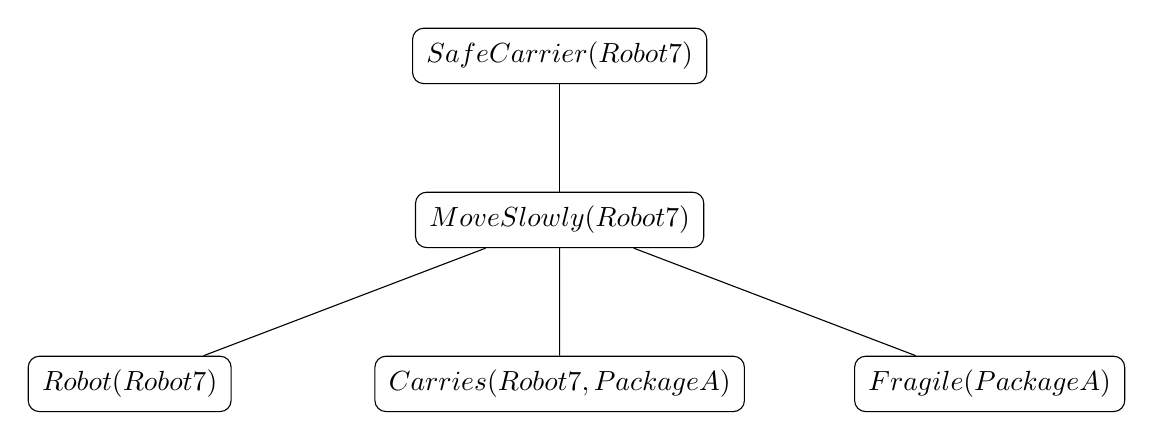
\begin{tikzpicture}[level distance=0.82in,sibling distance=2.15in,every node/.style={draw,rounded corners,align=center,inner sep=5pt}]
      \node {$SafeCarrier(Robot7)$}
        child {node {$MoveSlowly(Robot7)$}
          child {node {$Robot(Robot7)$}}
          child {node {$Carries(Robot7,PackageA)$}}
          child {node {$Fragile(PackageA)$}}
        };
    \end{tikzpicture}
  \end{center}

  \begin{keyidea}
    Backward chaining is goal-directed search through rules, with unification determining which branches are applicable.
  \end{keyidea}
\end{frame}

% -----------------------------------------------------------------------------
% Slide 38
% -----------------------------------------------------------------------------
\begin{frame}[shrink=10]{Forward vs. Backward Chaining in FOL}
  \begin{center}
    \renewcommand{\arraystretch}{1.35}
    \begin{tabular}{l|p{0.36\textwidth}|p{0.36\textwidth}}
      & \textbf{Forward chaining} & \textbf{Backward chaining} \\\hline
      Direction & Facts $\rightarrow$ consequences & Query $\rightarrow$ supporting premises \\
      Style & Data-driven & Goal-driven \\
      Uses unification to & Match rule premises & Match rule conclusions \\
      Best when & Many consequences matter & A specific query matters \\
      Search risk & Too many derived facts & Repeated / looping subgoals \\
    \end{tabular}
  \end{center}

  \begin{keyidea}
    Both methods use the same logical machinery; they differ mainly in where the search begins.
  \end{keyidea}
\end{frame}

\section{Practical Issues and Connections}

% -----------------------------------------------------------------------------
% Slide 39
% -----------------------------------------------------------------------------
\begin{frame}[shrink=10]{Variable Names Are Local: Standardize Apart}
  Two rules might both use the variable name $x$:
  \[
    Student(x) \rightarrow HasID(x)
  \]
  \[
    Employee(x) \rightarrow HasBadge(x).
  \]

  The two $x$ symbols are independent placeholders, not automatically the same object.

  In inference procedures we often rename variables before combining rules:
  \[
    x \mapsto x_1,\qquad x \mapsto x_2.
  \]

  \begin{keyidea}
    Standardizing variables apart prevents accidental collisions between unrelated rule instances.
  \end{keyidea}
\end{frame}

% -----------------------------------------------------------------------------
% Slide 40
% -----------------------------------------------------------------------------
\begin{frame}[shrink=10]{First-Order Inference Can Still Blow Up}
  \begin{columns}[T,onlytextwidth]
    \begin{column}{0.54\textwidth}
      Even compact rules may generate a large search space.
      \begin{itemize}
        \item Many facts may unify with the same premise.
        \item Multiple rule chains may prove the same goal.
        \item Recursive rules can create loops.
        \item Function symbols can generate endlessly deeper terms.
      \end{itemize}
    \end{column}
    \begin{column}{0.40\textwidth}
      \lectureimage[2.65in]{slide40.png}
    \end{column}
  \end{columns}
  \begin{keyidea}
    FOL is compact to write, but inference still behaves like search---and search needs control strategies.
  \end{keyidea}
\end{frame}

% -----------------------------------------------------------------------------
% Slide 41
% -----------------------------------------------------------------------------
\begin{frame}[shrink=10]{This Is the Core Idea Behind Logic Programming}
  Languages such as Prolog operationalize this style of reasoning:
  \begin{itemize}
    \item facts are stored symbolically;
    \item rules contain variables;
    \item queries trigger goal-directed proof search;
    \item unification matches goals to facts and rule heads.
  \end{itemize}

  \lectureimage[1.65in]{slide41.png}

  \begin{keyidea}
    In logic programming, computation itself can be viewed as proving that a query follows from a knowledge base.
  \end{keyidea}
\end{frame}

% -----------------------------------------------------------------------------
% Slide 42
% -----------------------------------------------------------------------------
\begin{frame}[shrink=10]{The Whole Logic Unit in One Pipeline}
  \begin{center}
    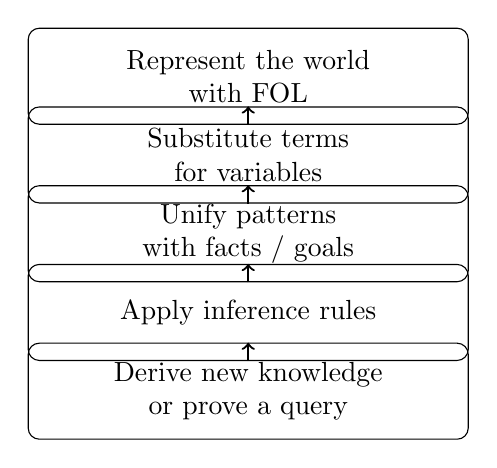
\begin{tikzpicture}[every node/.style={draw,rounded corners,align=center,minimum width=2.2in,minimum height=0.48in}]
      \node (rep) at (0,0) {Represent the world\\with FOL};
      \node (sub) at (0,-1.0) {Substitute terms\\for variables};
      \node (uni) at (0,-2.0) {Unify patterns\\with facts / goals};
      \node (inf) at (0,-3.0) {Apply inference rules};
      \node (new) at (0,-4.0) {Derive new knowledge\\or prove a query};
      \draw[->,thick] (rep)--(sub);
      \draw[->,thick] (sub)--(uni);
      \draw[->,thick] (uni)--(inf);
      \draw[->,thick] (inf)--(new);
    \end{tikzpicture}
  \end{center}

  \begin{keyidea}
    Knowledge representation gives the agent a language; unification and inference give that language computational force.
  \end{keyidea}
\end{frame}

% -----------------------------------------------------------------------------
% Slide 43
% -----------------------------------------------------------------------------
\begin{frame}[shrink=10]{Takeaways}
  \begin{itemize}
    \item A substitution maps variables to terms and instantiates general expressions.
    \item Unification finds a consistent substitution that makes two expressions identical.
    \item The most general unifier makes only the bindings required by the match.
    \item Generalized Modus Ponens combines unification with first-order rules.
    \item Forward chaining is data-driven; backward chaining is goal-driven.
    \item Both turn logical inference into a structured search problem over rules and substitutions.
  \end{itemize}

  \begin{keyidea}
    The machine does not ``understand'' that Socrates is mortal by intuition---it gets there by matching structure, binding variables, and applying a valid inference rule.
  \end{keyidea}
\end{frame}

\end{document}
